%%%%%%%%%%%%%%%%%%%%%%%%%%%%%%%%%%%%%%%%%
% Engineering Calculation Paper
% LaTeX Template
% Version 1.0 (20/1/13)
%
% This template has been downloaded from:
% http://www.LaTeXTemplates.com
%
% Original author:
% Dmitry Volynkin (dim_voly@yahoo.com.au)
%
% License:
% CC BY-NC-SA 3.0 (http://creativecommons.org/licenses/by-nc-sa/3.0/)
%
%%%%%%%%%%%%%%%%%%%%%%%%%%%%%%%%%%%%%%%%%

%----------------------------------------------------------------------------------------
%	PACKAGES AND OTHER DOCUMENT CONFIGURATIONS
%----------------------------------------------------------------------------------------

\documentclass[10pt,a4paper]{article} % Use A4 paper with a 12pt font size - different paper sizes will require manual recalculation of page margins and border positions

\usepackage{marginnote} % Required for margin notes
\usepackage{wallpaper} % Required to set each page to have a background
\usepackage{lastpage} % Required to print the total number of pages
\usepackage[left=1.3cm,right=4.6cm,top=1.8cm,bottom=4.0cm,marginparwidth=3.4cm]{geometry} % Adjust page margins
\usepackage{amsmath} % Required for equation customization
\usepackage{amssymb} % Required to include mathematical symbols
\usepackage{xcolor} % Required to specify colors by name
\usepackage{listings}

\usepackage{fancyhdr} % Required to customize headers
\setlength{\headheight}{80pt} % Increase the size of the header to accommodate meta-information
\pagestyle{fancy}\fancyhf{} % Use the custom header specified below
\renewcommand{\headrulewidth}{0pt} % Remove the default horizontal rule under the header

\setlength{\parindent}{0cm} % Remove paragraph indentation
\newcommand{\tab}{\hspace*{2em}} % Defines a new command for some horizontal space

\newcommand\BackgroundStructure{ % Command to specify the background of each page
\setlength{\unitlength}{1mm} % Set the unit length to millimeters

\definecolor{amaranth}{rgb}{0.9, 0.17, 0.31}
\definecolor{babyblueeyes}{rgb}{0.63, 0.79, 0.95}
\definecolor{beige}{rgb}{0.96, 0.96, 0.86}
\definecolor{bittersweet}{rgb}{1.0, 0.44, 0.37}
\definecolor{black}{rgb}{0.0, 0.0, 0.0}
\definecolor{bleudefrance}{rgb}{0.19, 0.55, 0.91}
\definecolor{bostonuniversityred}{rgb}{0.8, 0.0, 0.0}
\definecolor{brightube}{rgb}{0.82, 0.62, 0.91}
\definecolor{darkseagreen}{rgb}{0.56, 0.74, 0.56}
\definecolor{lavender}{rgb}{0.9, 0.9, 0.98}
\definecolor{mayablue}{rgb}{0.45, 0.76, 0.98}
\definecolor{cadmiumgreen}{rgb}{0.0, 0.42, 0.24}
\definecolor{almond}{rgb}{0.94, 0.87, 0.8}
\definecolor{antiquewhite}{rgb}{0.98, 0.92, 0.84}
\definecolor{ashgrey}{rgb}{0.7, 0.75, 0.71}
\definecolor{babyblueeyes}{rgb}{0.63, 0.79, 0.95}
\definecolor{beige}{rgb}{0.96, 0.96, 0.86}
\definecolor{blond}{rgb}{0.98, 0.94, 0.75}
\definecolor{cream}{rgb}{1.0, 0.99, 0.82}
\definecolor{eggshell}{rgb}{0.94, 0.92, 0.84}

\setlength\fboxsep{0mm} % Adjusts the distance between the frameboxes and the borderlines
\setlength\fboxrule{0.5mm} % Increase the thickness of the border line
\put(10, 10){\fcolorbox{black}{darkseagreen!10}{\framebox(155,247){}}} % Main content box
\put(165, 10){\fcolorbox{black}{blond!10}{\framebox(37,247){}}} % Margin box
\put(10, 262){\fcolorbox{black}{amaranth!10}{\framebox(192, 25){}}} % Header box
\put(170, 263){
\includegraphics[height=23mm,keepaspectratio]{csm}} % Logo box - maximum height/width: 
}

%----------------------------------------------------------------------------------------
%	HEADER INFORMATION
%----------------------------------------------------------------------------------------

\fancyhead[L]{
\begin{tabular}{l l | l l} % The header is a table with 4 columns
\textbf{CSC447:} & Parallel Programming &  \textbf{Name:} & Pia Chouayfati  \\ % Project name and page count
\textbf{Lab 1:}  & Pthreads &   \textbf{ID:}  & 201504706 \\ % Project name and page count
\textbf{Date:}&   \today &  \textbf{Page:} & \thepage/\pageref{LastPage}  \\ % Project name and page count
\textbf{Spring 2022} & & & \\ % Version and reviewed date
\end{tabular}}

 

%&  & \textbf{Date} & 27/11/2012 \\ % Job number and last updated date


%----------------------------------------------------------------------------------------

\begin{document}

\AddToShipoutPicture{\BackgroundStructure} % Set the background of each page to that specified above in the header information section

%----------------------------------------------------------------------------------------
%	DOCUMENT CONTENT
%----------------------------------------------------------------------------------------

\subsection*{Abstract}
Given the source code for calculating pi using pthreads, the serial code is reproduced and stats are recorded for both the serial and parallelized code. 

\section{Serial Code}

Below is the code reproduced serially (pi\_serial.c)

\begin{lstlisting}[language=C, caption=Serial code]
#include <stdio.h>
#include <stdlib.h>
#include <math.h>
#include <time.h>
#define STEPS 100000000
#define STEP_SIZE 1.0/STEPS

double calculate_pi()
{
    double lower = 0.5 * STEP_SIZE; 
    double higher = 1; //1/N, 2/N... N/N--->1
    double sum = 0;
    //while fraction is less than 1 
    while(lower < higher)
    {
        sum = sum + (STEP_SIZE * sqrt(1 - lower*lower));
        lower = lower + STEP_SIZE;
    }
    return sum*4;
}
int64_t millis()
{   struct timespec now;
    timespec_get(&now, TIME_UTC);
    return ((int64_t) now.tv_sec) * 1000 + 
    ((int64_t) now.tv_nsec) / 1000000;
}
int main()
    {   int64_t start = millis();
        double sum = calculate_pi();
        int64_t end = millis();

        printf("Reference PI = %.10lf 
        Computed PI = %.10lf\n", M_PI, sum);
        printf("Difference to Reference is 
        %.10lf\n", M_PI - sum);
        double time_elapsed = (end - start);
        printf("Time: %f ms\n", time_elapsed);
    }

\end{lstlisting}

\section{Time elapsed calculation}

Time was calculated in milliseconds using a custom function \textit{millis()} which utilizes \textit{timespec} and \textit{timespec\_get} and returns current time in milliseconds. A variable \textit{start} records the time upon execution, and a variable \textit{end} records it after execution. Time elapsed is the difference between the two. 

\begin{lstlisting}[language=C, caption=Getting time elapsed in ms]

int64_t millis()
{
    struct timespec now;
    timespec_get(&now, TIME_UTC);
    return ((int64_t) now.tv_sec) * 1000 + 
    ((int64_t) now.tv_nsec) / 1000000;
}

        int64_t start = millis();

<EXECUTE CODE>

        int64_t end = millis();
        
    double time_elapsed = (end - start);


\end{lstlisting}



\section{Results}

\subsubsection{Sequential code}

\begin{table}[h]
\begin{center}
\begin{tabular}{|l||l|l|l|}
\hline
Array Size & Runtime (in ms) & Pi value & Pi difference\\
\hline
1000 & 0 & 3.1416035449 & -0.0000108913 \\
10000 & 1 & 3.1415929980 & -0.0000003444 \\
100000 & 1 & 3.1415926645 & -0.0000000109 \\
1000000 & 5 & 3.1415926539 & -0.0000000003 \\
10000000 & 44 & 3.1415926542 & -0.0000000006 \\
100000000 & 383 & 3.1415926483 & 0.0000000053 \\
\hline
\end{tabular}
\end{center}
\caption{Results when running the sequential code with different array sizes}
\end{table}

\subsubsection{Parallelized code}

\begin{table}[h]
\begin{center}
\begin{tabular}{|l||l|l|l|}
\hline
Array Size & Runtime (in ms) & Pi value & Pi difference\\
\hline
1000 & 0 & 3.1416035449 & -0.0000108913 \\
10000 & 0 & 3.1415929980 & -0.0000003444 \\
100000 & 0 & 3.1415926645 & -0.0000000109 \\
1000000 & 2 & 3.1415926539 & -0.0000000003 \\
10000000 & 19 & 3.1415926542 & -0.0000000007 \\
100000000 & 197 & 3.1415926475 & 0.0000000061 \\
\hline
\end{tabular}
\end{center}
\caption{Results when running the pthread-parallelized code with different array sizes}
\end{table}


\section{Plotting}

The python library matplotlib was used for plotting in a jupyter notebook. Runtime was plotted against array size. The blue line represents the sequential code, the orange represents the parallelized code, as shown in the plot legend.

\begin{lstlisting}[language=Python, caption=Plotting]
import matplotlib.pyplot as plt

plt.xlabel('array size')
plt.ylabel('runtime (ms)')

#serial
plt.plot([1000, 10000, 100000, 1000000, 10000000, 100000000], 
[0, 1, 1, 5, 44, 383], label="sequential")

#pthreads
plt.plot([1000, 10000, 100000, 1000000, 10000000, 100000000], 
[0, 0, 0, 2, 19, 197], label="pthreads")

plt.title('runtime as a function of array size 
for sequential and parallelized code')
# legend
plt.legend()
# Display figure
plt.show()

\end{lstlisting}

\section{Discussion}

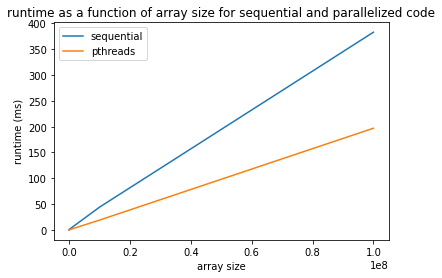
\includegraphics{lab_report/plot.png}

As shown in the plot, obviously the parallelized code outperforms the sequential code, executing in less time for the same array size. 
(Array size is shown in a logarithmic scale).
In general, as input size the time increases and the difference between  computed and actual Pi value decreases. Accuracy increases for a larger input value. However, as shown in the tables, 10000000 seems to be the appropriate input size. For larger inputs, we see the calculated pi value drift away from the actual value, to the other direction.


%----------------------------------------------------------------------------------------

\end{document}